%Here is the command to refer to another element (section, figure, table, ...) in the document: \emph{As discussed in Section~\ref{sect:overview} and as shown in Figure~\ref{fig:class-general}, ...}. Here is how to introduce a bibliographic citation~\cite{DAM}. Bibliographic references should be included in a \texttt{.bib} file. 
%Table generation is a bit complicated in Latex. You will soon become proficient, but to start you can rely on tools or external services. See for instance this \href{https://www.tablesgenerator.com}{https://www.tablesgenerator.com}. 

\subsection{Product perspective}

As for the SafeStreets system, the domain model is described in the diagram shown in Figure~\ref{fig:class-general}. Note that the diagram is not a complete description of the system, but rather a simplified version for easier understanding.

\begin{figure}[!h]
\centering
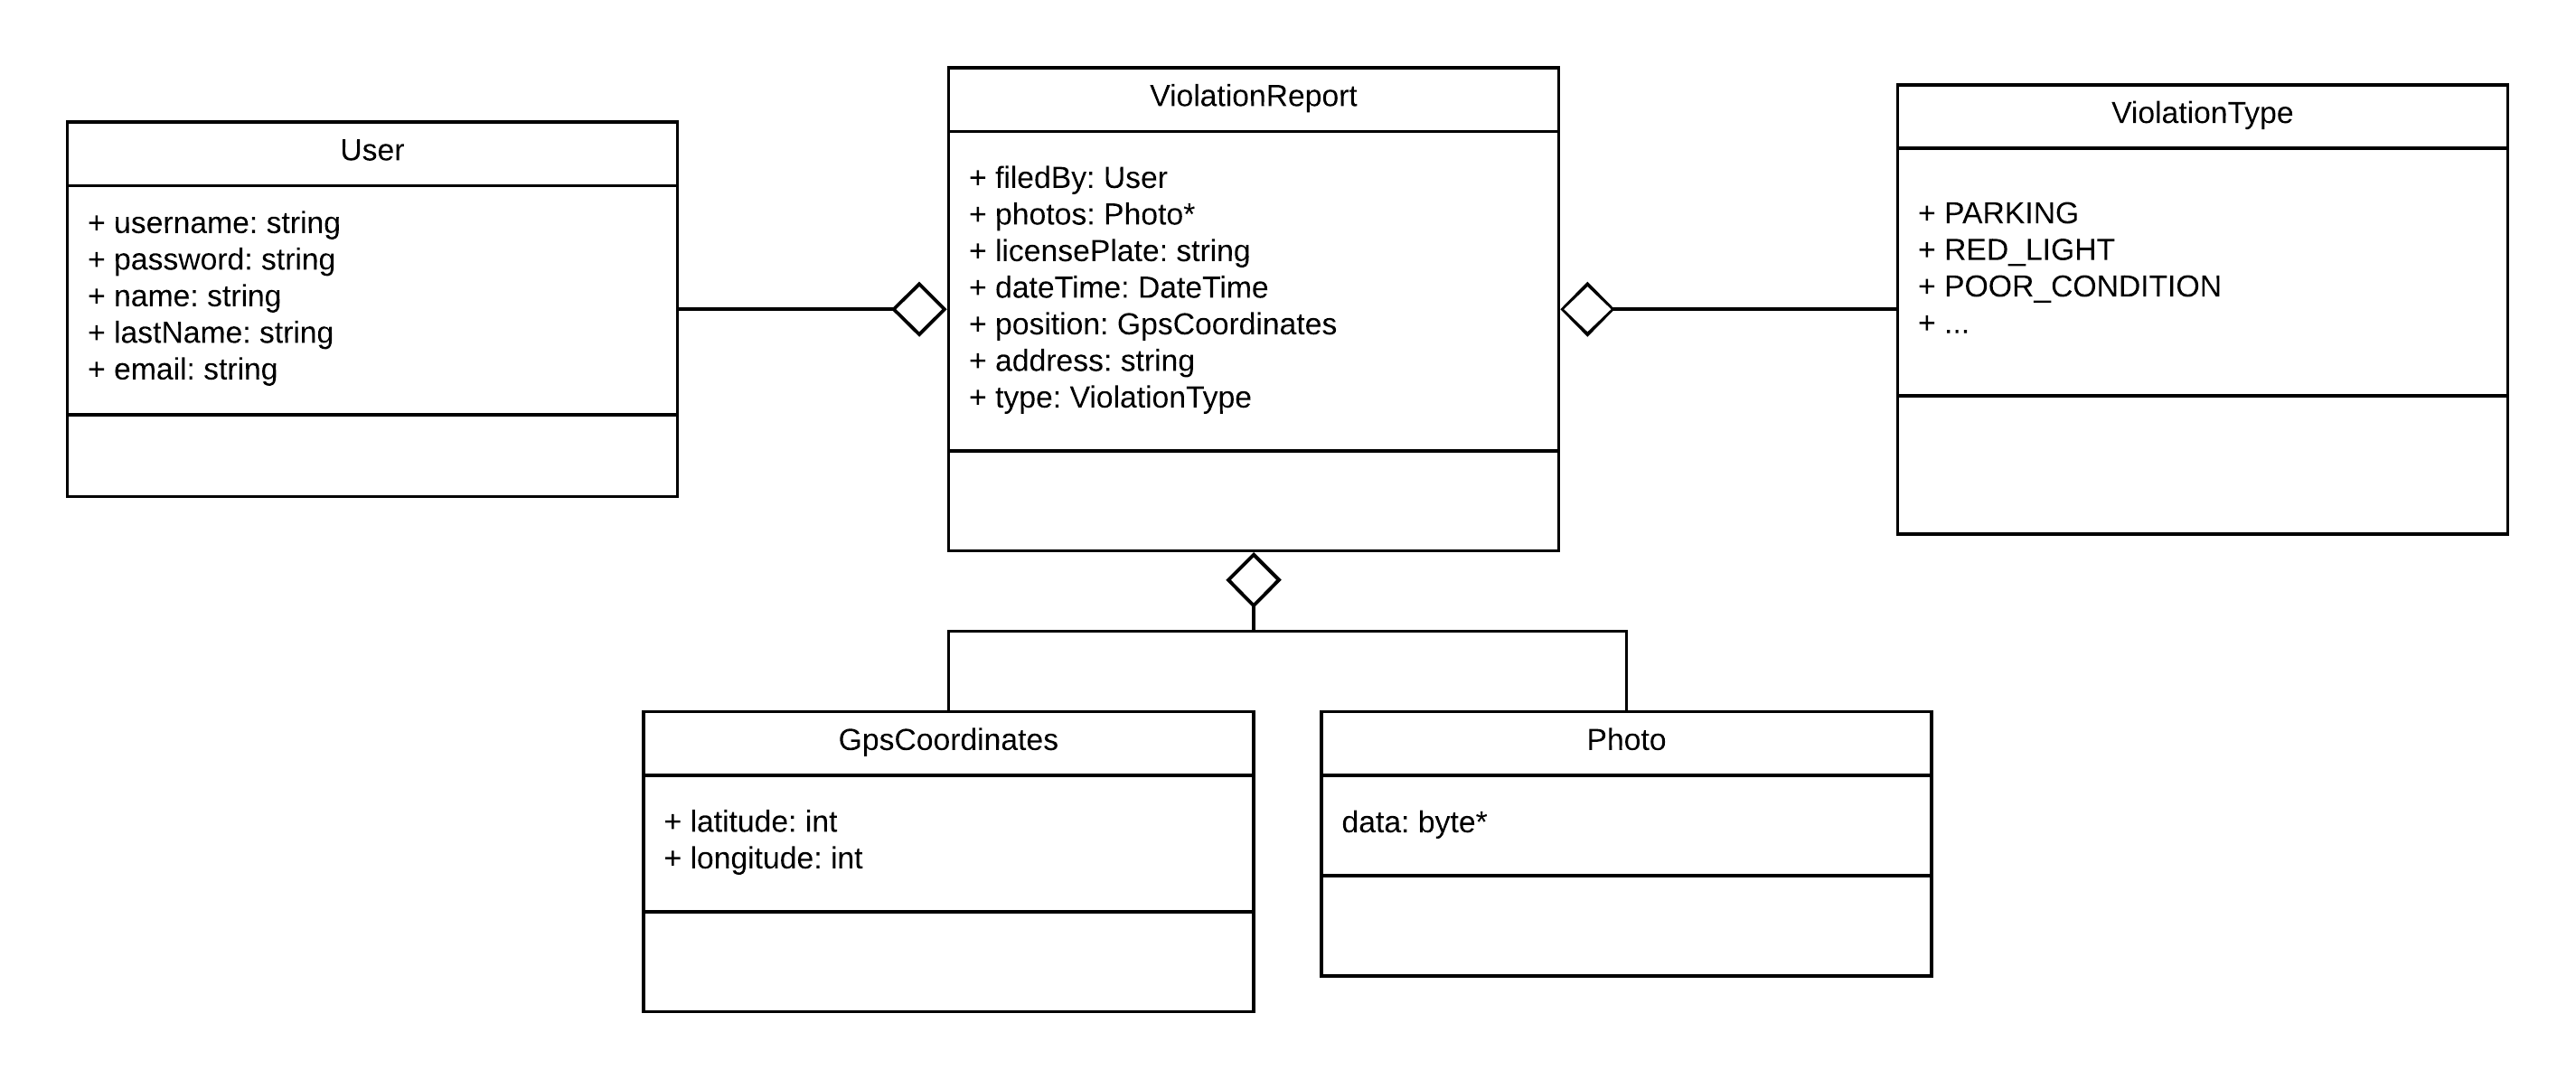
\includegraphics[width=\textwidth]{Images/class-general.png}
\caption{\label{fig:class-general}Class diagram.}
\end{figure}

Inspecting the class diagram, we can see that most of the system revolves around the violation reports and their processing, this is the core of the system.
In the state diagram shown in Figure~\ref{fig:state-report-submission}, the process of submitting a report is explained.

\begin{figure}[!h]
\centering
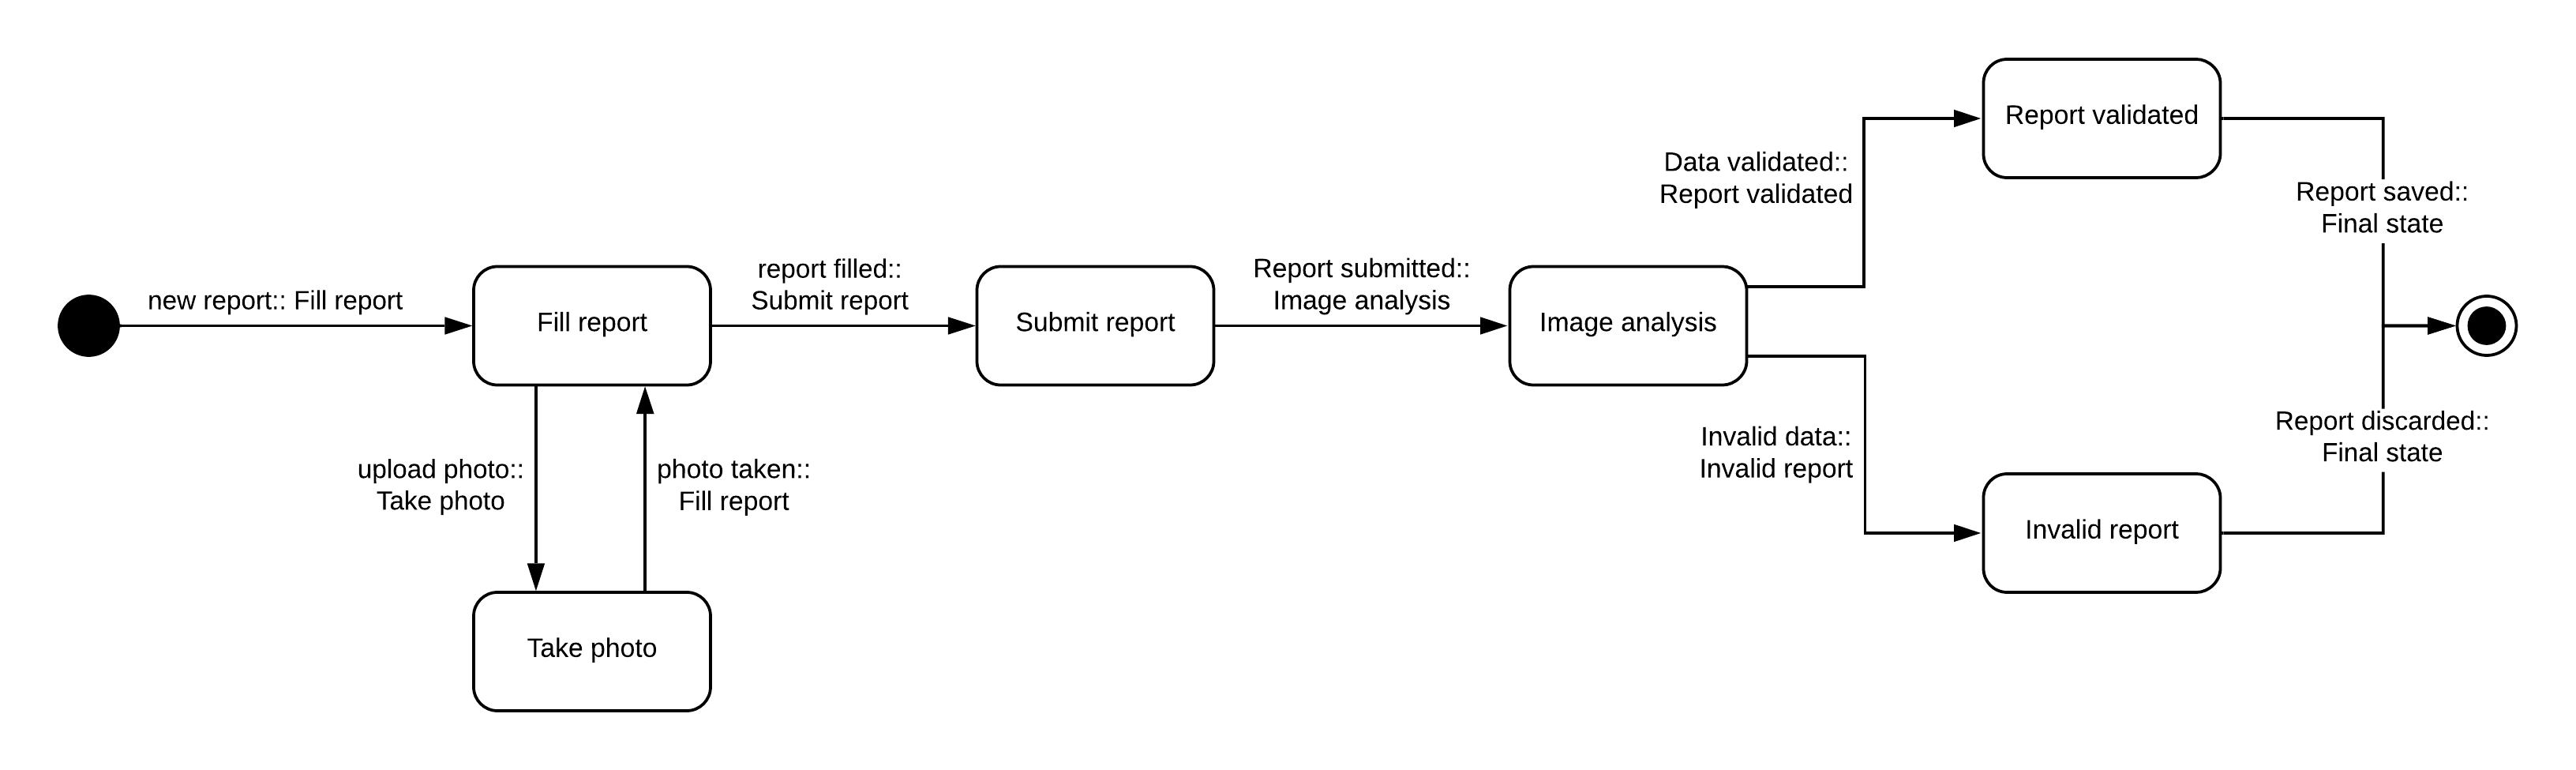
\includegraphics[width=\textwidth]{Images/state-report-submission.png}
\caption{\label{fig:state-report-submission}State diagram - Report submission.}
\end{figure}

As observed in the diagram, for submitting a report, the user is first required to fill a formulary with the required information and photo. After the submission, the SafeStreets system executes an analysis of the data, matching it with the provided image. This can result in either a invalid or a valid report. An invalid report is discarded, with possible measures taken against the account that submitted it. A valid report is saved in the database. When the report is saved, it is made available for the different users to query, either through the mobile application or through the public API.

\subsection{Product functions}
The functionality of the system can be divided into three groups. In the following section, these functions are listed and explained, taking into account the already specified goals of the system.

\subsubsection{Violation report}
The reporting of violations is the main functionality of the system. It allows its registered users to submit a traffic violation report. The user is required to provide data, such as a picture of the violation, the license plate of the vehicle committing the violation and the type of violation. On top of this information, the mobile application will provide the system with metadata which includes the gps location, date and time of the report.
After the submission, the system analyses the provided information, checking its integrity. If the report is considered invalid or to have been compromised, it is discarded and the user is flagged as not trustworthy. Otherwise, the report is saved and made available to the rest of the system.

\subsubsection{Image analysis}
In order to confirm the validity of a report, the system performs an analysis of the submitted image. The picture is expected to show the vehicle committing the violation along with a clear view of its license plate. The analysis searches the image for this information and matches the detected license plate with the one provided in the report.

\subsubsection{Data querying}
Gathered information by SafeStreets can be accessed by all users. There are two ways in which the data can be accessed, via the mobile application or through the public API.
In the first case, the mobile application provides users with the ability to see violations in a map, allowing the user to also filter these violations by date and type. 
On the other hand, the API allows for SafeStreets to be integrated with other third party systems. Users are able to query the available data according to their role and obtain the information in an analysis-friendly format.

\subsection{User characteristics}
The actors identified as the users of the application are:
\begin{itemize}
\item
User: A person that has registered to SafeStreets and is capable of reporting violations. 
\item
Municipality system: A system belonging to the municipality that communicates with SafeStreets through the exposed API. Capable of accessing more information than the standard user.
\item
Administrator: An employee of SafeStreets that maintains and updates the system.
\end{itemize}

\subsection{Assumptions, dependencies and constraints}

\begin{itemize}
\item
[D1] - An accurate gps location can be acquired from the device the user is running SafeStreets on.
\item
[D2] - The device running SafeStreets has a camera.
\item
[D3] - A violation report cannot be canceled
\item
[D4] - The metadata of the picture in the violation report is accurate
\item
[D5] - There is a system available capable of connecting a license plate to characteristics of the car (make, model, color)
\end{itemize}




